\pdfinfoomitdate=1
\pdftrailerid{}
\documentclass[12pt]{article}
\usepackage[letterpaper,margin=0.65in,headheight=16pt,headsep=18pt,footskip=25pt]{geometry}
\usepackage{tikz,amsmath,array,fancyhdr}
\usetikzlibrary{arrows.meta,patterns}
\usepackage[T1]{fontenc}
\usepackage{lmodern}
\renewcommand{\familydefault}{\sfdefault}
\pagestyle{fancy}\fancyhf{}
\fancyhead[L]{\small Week 89 / Growing shapes and totals / Grades K--5}
\fancyfoot[L]{\small Bellingham Math Circle / Week 89 / W89-M-v2}
\fancyfoot[R]{\small\thepage}
\renewcommand{\headrulewidth}{0.4pt}\renewcommand{\footrulewidth}{0pt}
\setlength{\parindent}{0pt}\setlength{\parskip}{9pt}
\newcommand{\problem}[2]{\textbf{Problem #1:} #2\par}
\newcommand{\answer}[1]{\par\vspace{#1}\par}
\newcommand{\tile}[3]{\filldraw[fill=#3,draw=black!65,line width=.35pt] (#1,#2) rectangle ++(1,1);}
\newcommand{\squarefig}[1]{\begin{tikzpicture}[x=5mm,y=5mm,baseline=(current bounding box.center)]\foreach \x in {1,...,#1}{\foreach \y in {1,...,#1}{\tile{\x}{\y}{white}}}\end{tikzpicture}}
\newcommand{\stairfig}[1]{\begin{tikzpicture}[x=5mm,y=5mm,baseline=(current bounding box.center)]\foreach \y in {1,...,#1}{\foreach \x in {1,...,\y}{\tile{\x}{#1-\y}{white}}}\end{tikzpicture}}
\newcommand{\rectfig}[1]{\begin{tikzpicture}[x=5mm,y=5mm,baseline=(current bounding box.center)]\pgfmathtruncatemacro{\w}{#1+1}\foreach \x in {1,...,\w}{\foreach \y in {1,...,#1}{\tile{\x}{\y}{white}}}\end{tikzpicture}}
\newcommand{\slips}[1]{\begin{tikzpicture}[baseline=(current bounding box.center)]\foreach \a [count=\i from 0] in {#1}{\draw (\i*1.1,0) rectangle ++(.85,.75);\node at (\i*1.1+.425,.375){\Large\a};}\end{tikzpicture}}
\newcommand{\tray}[4]{\draw[rounded corners=3pt] (#1,#2) rectangle ++(1.65,1.15);\node at (#1+.825,#2+.63){\Large #4};\node[font=\small] at (#1+.825,#2-.25){#3};}
\begin{document}
\begin{center}\begin{tikzpicture}[x=1mm,y=1mm]
\draw[line width=.8pt] (0,0) rectangle (120,120);
\draw[step=20,black!40,line width=.3pt] (0,0) grid (120,120);
\node[below] at (60,-4){120 mm $\times$ 120 mm};
\draw (0,-22)--(20,-22);\draw (0,-20)--(0,-24);\draw (20,-20)--(20,-24);
\node[below] at (10,-25){20 mm};
\end{tikzpicture}\end{center}
\vspace{3mm}
\begin{center}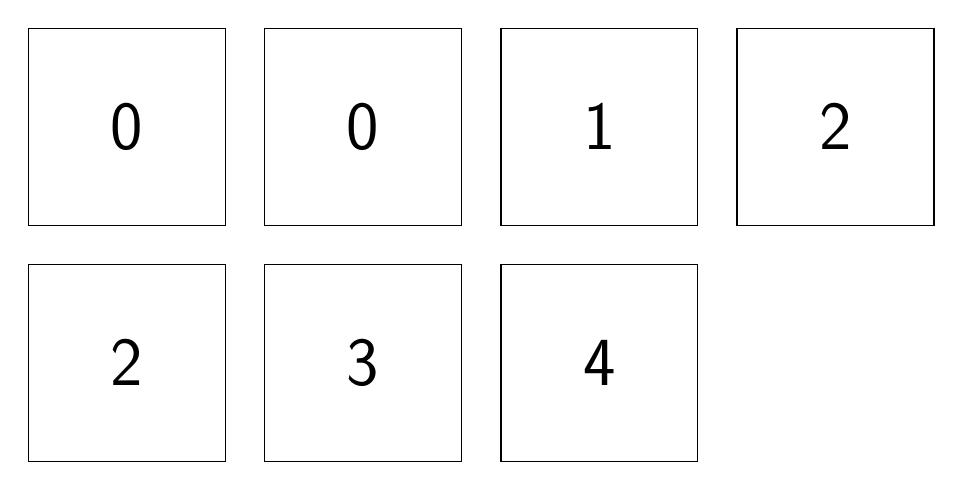
\begin{tikzpicture}[x=1mm,y=1mm]
\foreach \val/\xx/\yy in {0/0/30,0/30/30,1/60/30,2/90/30,2/0/0,3/30/0,4/60/0}{
\draw[line width=.5pt] (\xx,\yy) rectangle ++(25,25);
\node[font=\Huge] at (\xx+12.5,\yy+12.5){\val};
}
\end{tikzpicture}\end{center}
\newpage
\begin{center}\begin{tikzpicture}[x=1mm,y=1mm]
\draw[line width=.8pt] (0,0) rectangle (140,120);
\draw[step=20,black!40,line width=.3pt] (0,0) grid (140,120);
\node[below] at (70,-4){140 mm $\times$ 120 mm};
\draw (0,-22)--(20,-22);\draw (0,-20)--(0,-24);\draw (20,-20)--(20,-24);
\node[below] at (10,-25){20 mm};
\end{tikzpicture}\end{center}
\vspace{3mm}
\begin{center}\begin{tikzpicture}[x=1mm,y=1mm]
\foreach \xx in {0,55,110}{\foreach \yy in {0,30}{
\draw[line width=.5pt] (\xx,\yy) rectangle ++(50,25);
\node[font=\footnotesize,anchor=north west] at (\xx+2,\yy+24){total};
}}
\end{tikzpicture}\end{center}\end{document}
